
\section{Zielsetzung}
Das Ziel des Versuches ist, dass Elastizitätsmodul verschiedener Metalle und
Legierungen zu messen. %und mit Literaturwerten zu vergleichen
\section{Theorie}
\label{sec:Theorie}
Wirken Spannungen auf eine Oberfläche eines Körpers, so können Änderungen an
Gestalt und Volumen enstehen. Dabei werden die Komponenten der Spannungen die
senkrecht zur Oberfläche stehen als Normalspannung $\sigma$ oder Druck und die
parallelen als Tangential-oder Schubspannung bezeichnet. Ist nun die relative
Änderung $ \increment \symup{L /L} $ hinreichend klein, wobei L eine lineare Körperdimension
ist, so gibt das Hooksche Gesetz den Zusammenhang:
\begin{equation}
  \sigma = E\frac{\increment L}{L}.
  \label{eqn:hook}
\end{equation}
E bezeichnet dabei das Elastizitätsmodul.

\subsection{Biegung eines homogenen Stabes bei einseitiger Einspannung}
\label{sec:T1}
Ist ein Stab, der Länge L, an einer Seite eingespannt und es wirkt eine Kraft F
auf einen
Querschnitt Q des Stabes der den Abstand x von seiner Einspannung hat, wie in
Abbildung \ref{fig:abb2}, dann übt diese ein Drehmoment aus. Dieses Drehmoment
lenkt den Querschnitt Q aus seiner ursprünglichen vertikalen Lage aus. Dabei
wird die obere Schicht des Stabes gedehnt und die untere gestaucht. Da es sich
bei dem Stab um ein elastischen Körper handelt, tretten im inneren des Stabes
Spannungen auf, die der Auslenkung D(x) entgegenwirken.
\begin{figure}
  \centering
  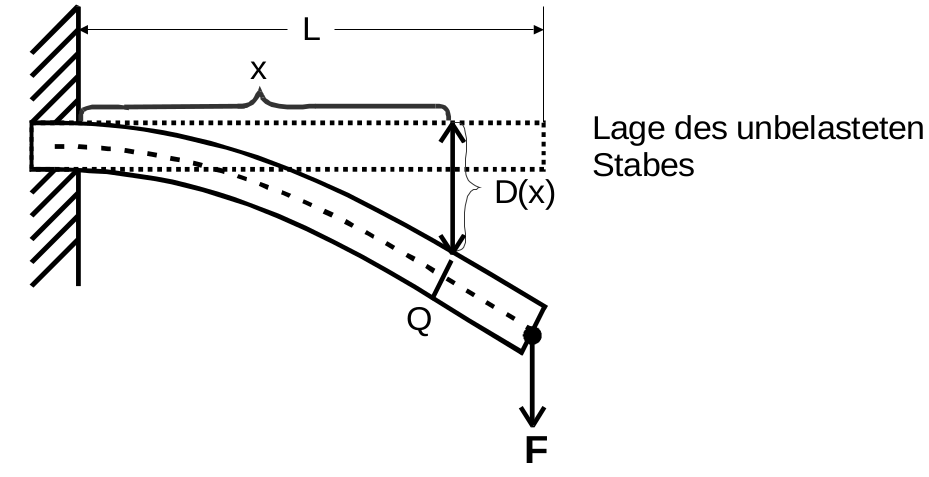
\includegraphics[height = 7cm]{logos/Abb2.png}
  \caption{Biegung eines elastischen Stabes bei einseitiger Einspannung
  aus Quelle \cite{Anleitung}}
  \label{fig:abb2}
\end{figure}
\FloatBarrier
Dazwischen gibt es eine Fläche, in der keine Spannungen auftretten und ihre
ursprüngliche Länge behält, diese wird neutrale Faser gennant und ist in
Abb.\ref{fig:abb2} als gestrichelte Linie innerhalb des Stabes eingezeichnet.
Daraus ergibt sich dann für die Auslenkung
\begin{equation}
  D(x) = \frac{F}{2EI} \left(Lx^2-
  \frac{x^3}{3}\right) \; \text{für} \; 0 \leq x \leq L.
  \label{eqn:D1}
\end{equation}
I in Gleichung \eqref{eqn:D1}, bezeichnet dabei das Flächenträgheitsmoment, dies
ist definiert durch:
\begin{equation}
  I \coloneq \int_{Q}{y}^2\symup{dq}(y).
  \label{eqn:I}
\end{equation}
Dabei ist y definiert als der Abstand des Flächenelemntes dq von der neutralen
Faser.
\subsection{Biegung eines homogenen Stabes bei beidseitiger Auflage}
\label{sec:T2}
Nun wird ein Stab an beiden Enden aufgelgt und in der Stabmitte
durch eine Kraft F durchgebogen, wie in Abbildung\ref{fig:abb5} zusehen. Hier
wirkt die Kraft F mit Hebelarm x am Querschnitt Q.
\begin{figure}
  \centering
  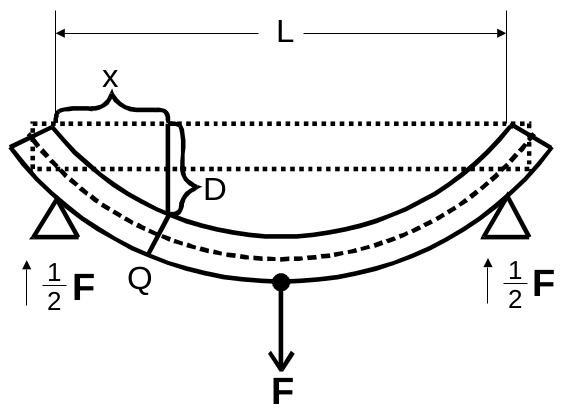
\includegraphics[height= 7cm]{logos/Abb5.png}
  \caption{Biegung eines elastischen Stabes bei zweiseitiger Auflage
  entnommen aus Quelle \cite{Anleitung} }
  \label{fig:abb5}
\end{figure}
\FloatBarrier
Dann ergibt sich für die Auslenkung:
\begin{equation}
  D(x) = \frac{F}{48 EI}
  \left( 3L^2 x-4x^3 \right) \; \text{für} \;
  0 \leq x \leq \frac{L}{2} .
  \label{eqn:D2}
\end{equation}
Für die rechte Stabhälfte mit D(L)$=$0 gilt dann:
\begin{equation}
  D(x) = \frac{F}{48 EI}
  \left(4 x^3 - 12 Lx^2 + 9 L^2x - L^3\right)
  \; \text{für} \; \frac{L}{2} \leq x \leq L .
  \label{eqn:D3}
\end{equation}
Auch hier ist bei beiden Gleichungen (\eqref{eqn:D2}\&\eqref{eqn:D3}) I das
Flächenträgheitsmoment aus Gleichung \eqref{eqn:I}.
